\documentclass{article}
\usepackage{amsmath}
\usepackage{tikz}
\usepackage{geometry}
\geometry{margin=2.5cm}
\usepackage{graphicx}
\usepackage{physics}
\usepackage{bm}

\title{Symbolische Darstellung der Beta-Korrekturfrequenz}
\author{}
\date{}

\begin{document}

\maketitle

\section*{Beta-Korrektur als fundamentale Frequenz}

Die aus der Optimierung der Beta-Skala resultierende Korrekturfrequenz
\[
\varepsilon = 0.00012151 \approx \frac{1}{8217} \approx \frac{4}{32901}
\]
kann mit hoher Präzision durch rationale Approximationen beschrieben werden.

\subsection*{Geometrischer Bezug: Einheitskreis in 33 Sektoren}

\begin{center}
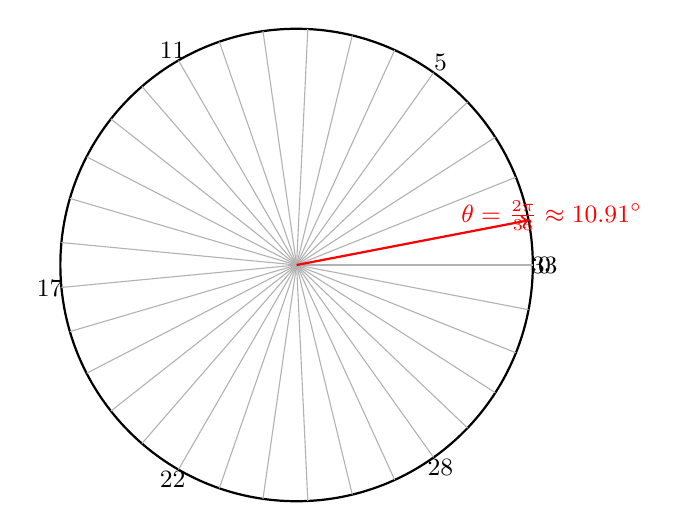
\begin{tikzpicture}[scale=3]
  % Kreis zeichnen
  \draw[thick] (0,0) circle(1);

  % 33 Teilungen
  \foreach \i in {1,...,33} {
    \draw[gray!60] (0,0) -- ({cos(360/33*\i)}, {sin(360/33*\i)});
  }

  % Beschriftung außen
  \foreach \i/\t in {0/0, 5/5, 11/11, 17/17, 22/22, 28/28, 33/33} {
    \draw ({1.05*cos(360/33*\i)}, {1.05*sin(360/33*\i)}) node {\small $\t$};
  }

  % Radius und Winkelbezug
  \draw[->, thick, red] (0,0) -- ({cos(360/33)}, {sin(360/33)});
  \node[red] at ({1.1*cos(360/33)}, {1.1*sin(360/33)}) {\small $\theta = \frac{2\pi}{33} \approx 10.91^\circ$};

\end{tikzpicture}
\end{center}

\subsection*{Interpretation}

\begin{itemize}
    \item $33$: Zahl der Spiralwindungen pro DNA-Helixumdrehung ($\approx 10.91^{\circ}$ pro Abschnitt)
    \item Die Beta-Korrekturfrequenz $\varepsilon$ spiegelt mögliche periodische Resonanzen auf dieser Skala wider
\end{itemize}

\subsection*{Bezeichnungsvorschlag}

\textbf{Freese-Beta-Korrekturfrequenz} oder \textbf{Fundamentale Skalenresonanz der Beta-Skala}

\end{document}